\chapter{Concepts}\label{chap:concepts}

The purpose of this chapter is to clarify the conceptual difference between our and other mainstream web applications. We start with standards and principles related to data organization and publishing on the modern Web. Then, different kinds of decentralized storage are covered concerning operational risks. Finally, we give an overview of \acs{solid} technology --- our choice for storing personal data.

\section{Linked Data}\label{sec:linked-data}

% https://www.w3.org/2001/sw/
% https://www.w3.org/RDF/FAQ/

The World Wide Web has gradually evolved into a dynamic and heterogeneous environment for social interactions, collaboration, and innovation. Consequently, the amount of available data has increased tremendously. It is safe to assume that no human, without the help of a machine, can organize them and uncover their hidden potential.

Suppose a user has published a photo without any attached metadata. Perhaps their friends and relatives would be able to understand the context of the picture and its value, but the same task does not appear so easy for an intelligent agent. The \emph{Semantic Web} is an extension of the standard ``Web of documents'' to give data additional dimension and enable machines to navigate resources, read and reason about them. This term was introduced by Tim Berners-Lee, the creator of the Web, long before the exponential data growth became an issue.

At first, this task may seem very ambitious, yet achievable if communicated through standards and recommendations, allowing other participants to contribute. As one might expect, the topic is indeed vast. Therefore, we discuss~only a subset relevant to this thesis. So, how can we make the Web machine-readable?

The initial step in the right direction is to provide a tool for describing data. The \ac{rdf}~\cite{rdfconcepts14} is an abstract syntax for representing information on the Web. It is well-suited for modeling structures similar to directed, labeled multigraphs. Every edge of a graph is a \emph{statement} --- a triple consisting of a subject, predicate, and object --- applicable in a given context. An \acs{rdf} document is a collection of \acs{rdf} graphs.

For example, the sentence \emph{``Alice knows Bob.''} can be expressed by the statement illustrated in Figure~\ref{fig:rdf-statement}, provided that additional information about entities is available upon dereferencing the corresponding links.

\begin{figure}[h!]
\centering
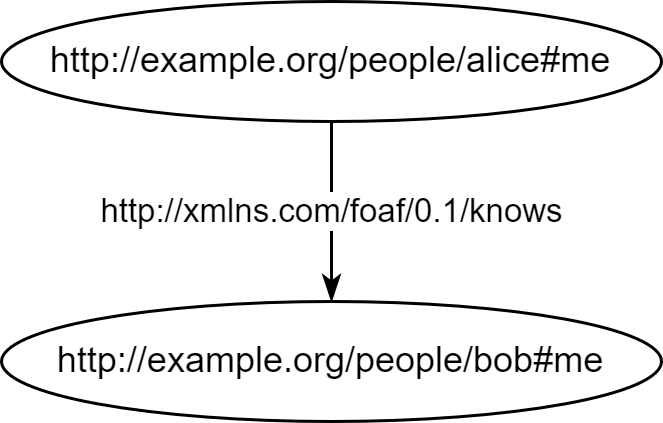
\includegraphics[width=0.45\linewidth]{img/concepts/rdf-statement.png}
\caption{An RDF graph with one triple.}
\label{fig:rdf-statement}
\end{figure}

There are multiple options to choose from while serializing \acs{rdf} data. Let us demonstrate two very different examples.

The most obvious ones are N-Triples~\cite{ntriples14} and N-Quads~\cite{nquads14}, that is to write each triple (optionally with a graph name) on a separate row. Reading one triple at a time is especially beneficial in case an \acs{rdf} document is large enough so that it does not fit into the main memory. An example of an \acs{rdf} statement serialized as N-Triple follows.

\begin{minted}{text}
<http://example.org/people/alice#me> <http://xmlns.com/foaf/0.1/knows> <http://example.org/people/bob#me> .
\end{minted}

\ac{jsonld}~\cite{jsonld20} is another option based on a well-known and widely used \ac{json} data format. Triples are contained within the \texttt{@graph} property. The \texttt{@context} defines a mapping between properties of a \acs{json} object and their corresponding links.

Our running example serialized into \acs{jsonld} is shown in the code snippet below, but it is important to note that this serialization is much more versatile.

\begin{minted}{text}
{
  "@context": {
    "knows": {
      "@id": "http://xmlns.com/foaf/0.1/knows",
      "@type": "@id"
    }
  },
  "@graph": [
    {
      "@id": "http://example.org/people/alice#me",
      "knows": "http://example.org/people/bob#me"
    }
  ]
}
\end{minted}

We have learned how to model data and represent them in a machine-readable form. The \ac{sparql}~\cite{sparql13} enables searching and modifying \acs{rdf} data via \emph{basic graph pattern matching}, \emph{property paths} and other advanced techniques.

The following query searches for all the people that Alice knows. If executed on our running example, the result would be a table with the only cell containing a link to Bob's web page.

\begin{minted}{text}
PREFIX foaf: <http://xmlns.com/foaf/0.1/>

SELECT * WHERE {
  <http://example.org/people/alice#me> foaf:knows ?o .
}
\end{minted}

Finally, we state four slightly adapted principles, so-called \emph{Linked Data}, proposed by Tim Berners-Lee~\cite{timbl06}. If properly followed, there is a chance that the Web will evolve into a standardized global-scale database.

\begin{enumerate}
\item Use \ac{iri} as names for things.
\item Use \acs{http}(S) \acs{iri}s so that people can look up those names.
\item When someone looks up an \acs{iri}, provide useful information in \acs{rdf}.
\item Include links to other \acs{iri}s, so that they can discover more things.
\end{enumerate}

\section{Reclaiming data}

Earlier, we mentioned operational risks that arise from centralized data management. The common reason behind all of them is that data are in the possession of a service provider. Let us discuss three very different kinds of \emph{decentralized storage} --- those not belonging to a service provider --- applicable in web development that could help to mitigate or even avoid these risks altogether.

\subsection*{Device storage}

The simplest approach is to use the file system of the device used to access a web page. The latest version of the application is fetched on page refresh. Then, it behaves more like being installed on a desktop computer.

Such storage provides control over where data are stored and ensures privacy, but it makes collaboration hard. There is no simple answer to how to access data from multiple devices either.

Kleppmann et al.~\cite{kleppman19} formulated seven principles of \emph{local-first software}. Their vision was to harness the benefits of the software-as-a-service business model but with the assumption that the application makes a local copy of all data and treats it as a primary replica. The user does not need to wait for actions to finish or be online all the time; changes made locally are eventually propagated to the cloud.

\subsection*{Peer-to-peer storage}

BitTorrent\footnote{\href{https://www.bittorrent.org/}{https://www.bittorrent.org/}}, IPFS\footnote{\href{https://ipfs.tech/}{https://ipfs.tech/}}, SAFE Network\footnote{\href{https://primer.safenetwork.org/}{https://primer.safenetwork.org/}}, and PingER~\cite{ali18} are examples of technologies based on peer-to-peer file sharing and communication protocols. Data~are split into chunks and replicated among agents available on the network; there is no single point of failure.

It is worth noting that p2p-storages are decentralized from the user's perspective as well, which brings additional challenges. Published data are hard or even impossible to alter. If not encrypted, distributed chunks may potentially be used in an unsolicited way. Therefore, additional measures for data protection might need to be considered upfront.

\subsection*{Personal storage}

The last group in our classification comprises technologies that enable users or system administrators to create a secure space for their data, decide the exact physical location of data, grant and revoke permissions to access resources, and so on. Individual spaces are interconnected and establish a federated network.

Mastodon\footnote{\href{https://mastodon.social/}{https://mastodon.social/}}, Diaspora\footnote{\href{https://diasporafoundation.org/}{https://diasporafoundation.org/}}, and Hubzilla\footnote{\href{https://hubzilla.org/}{https://hubzilla.org/}} are representatives of rather specialized software for social interactions, aiming to meet the needs of groups. Solid\footnote{\href{https://solidproject.org/}{https://solidproject.org/}} stands out as a technology for storing the personal data of individuals.

\vspace{0.5em}

Assuming that the service application does not perform unintended operations or act maliciously, personal storage offers the most flexibility concerning the risks we address. Furthermore, we do not attempt to implement a social network but focus on providing a novel way to search routes. Hence, \acs{solid} will be our choice for storing user data.

\section{Solid Project}\label{sec:solid-project}

% https://rubenverborgh.github.io/Web-Foundation-2018/
% https://rubenverborgh.github.io/WebFundamentals/decentralization/

\ac{solid}~\cite{solid22} is a specification built on top of the existing infrastructure and standards, and any \acs{solid}-compliant implementation acts as a personal storage we described in the previous section.

Started as a research project by Tim Berners-Lee and other collaborators in response to the improper use of the Web~\cite{timbl09}, the technology later developed into the startup Inrupt\footnote{\href{https://www.inrupt.com/}{https://www.inrupt.com/}} to turn \acs{solid} into a market-ready product.

Within \acs{solid}, user data are stored in personal online data stores called \emph{pods}, following the principles of \emph{\nameref{sec:linked-data}}. It distinguishes between structured \acs{rdf} datasets and unstructured binary blobs (text, images, etc.). Pods reside on a \emph{pod server} and are accessed via a well-defined \acs{http} \acs{api}. Servers are also responsible for authentication, authorization, access control, and request handling~\cite{mansour16}.

The concept of decentralization using \acs{solid} is shown in Figure~\ref{fig:concept-of-decentralization}. The owner of a pod can grant and revoke permissions based on unique user identifiers. Agents attempt to access a resource through \acs{solid} apps. Agent~1 is allowed, but Agent~N is not because their identifier does not appear in the list.

\begin{figure}[h!]
\centering
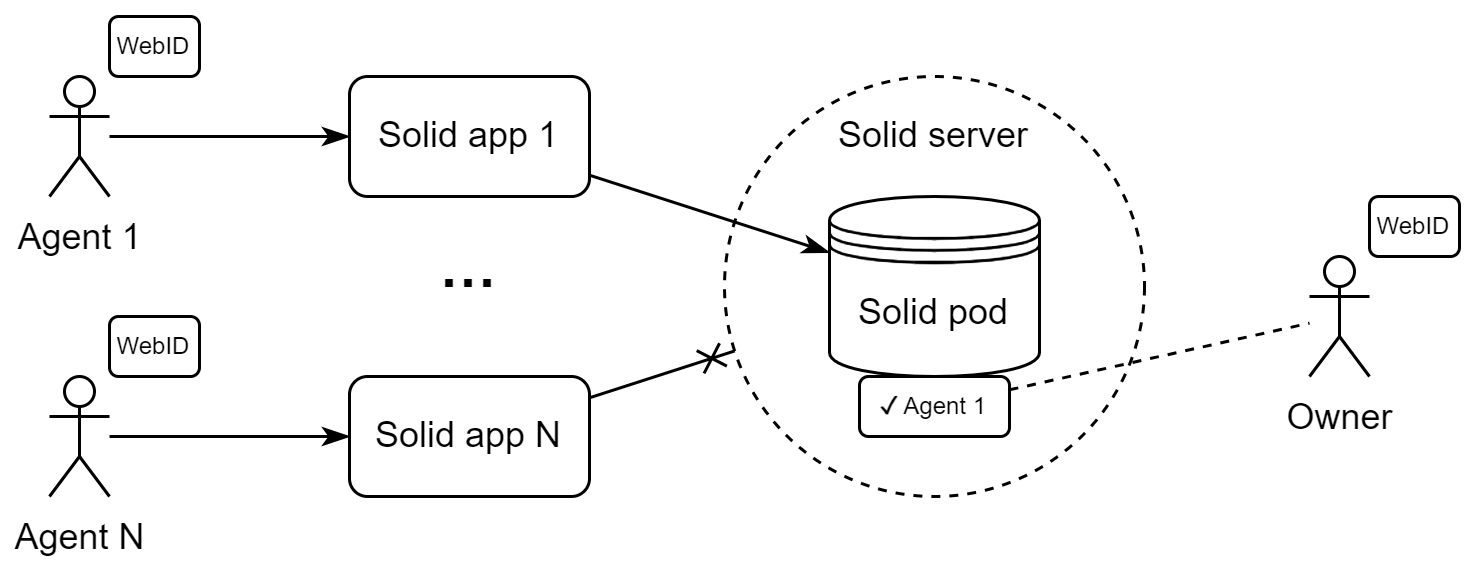
\includegraphics[width=0.75\linewidth]{img/concepts/concept-of-decentralization.png}
\caption{The concept of decentralization using Solid.}
\label{fig:concept-of-decentralization}
\end{figure}
